\section*{The knowledge that I got from the lecture}
\section*{Space}
\paragraph*{Space environment \& human life}: These days, we depend on the space systems such as communication satellites, broadcast satellites, meteorological satellites and global positioning system (GPS) satellites for many of our modern convenience and for navigation. The construction of the International Space Station and space travel planned by private sectors increse the potential of civillians visiting space. Many risks are associated with the environment in space, such as radiations hazards that astronauts face, single event upsets of electrical equipment on satellites, degradation of solar panels. In addition, geomagnetically induced currents associated with intense geomagnetic stroms sometimes cause problems on power grids on the Earth\cite{lecture}.\\
So we need to define what space environment is. the Space Environment is the region beginning at the lower boundary of the Earth's ionosphere (approximately 50 km) and extending outward that contains solid particles (asteroids and meteoroids), energetic charged particles (ions, protons, electrons, etc.), and electromagnetic and ionizing radiation (x-rays, extreme ultraviolet, gamma rays, etc.).\\
Now we see that the space environment effects to our earth and let's look a little about it. Before we begin we need to know the term "Space Weather". The Space Weather is the concept of changing environmental conditions in outer sapce. It is distinct from the concept of weather within a planetary atmosphere, and generally deals with the intersections of ambient radiation and matter within interplanetary, and occasionally interstellar space\cite{www.thefreedictionary.com2018}.\\
From the definition of the National Academy of Science: "Space weather describes the conditions in space that affect Earth and its technological systems. Our space weather is a consequence of the behavior of the sun, the nature of Earth's magnetic field, and our location in the solar system."\cite{lecture}.\\
Our earth is surrounded by the magnetic field that prevents radiation from the sun which is produced by the explosions at the sun. So it is very important to understand the behavior of the sun and the nature of the magnetic field. Figure \ref{fig:magField} shows the example of the earth's magnetic field. The measurements of plasma waves is one of the important thing to study in space environment.\\
\begin{figure}[h!]
  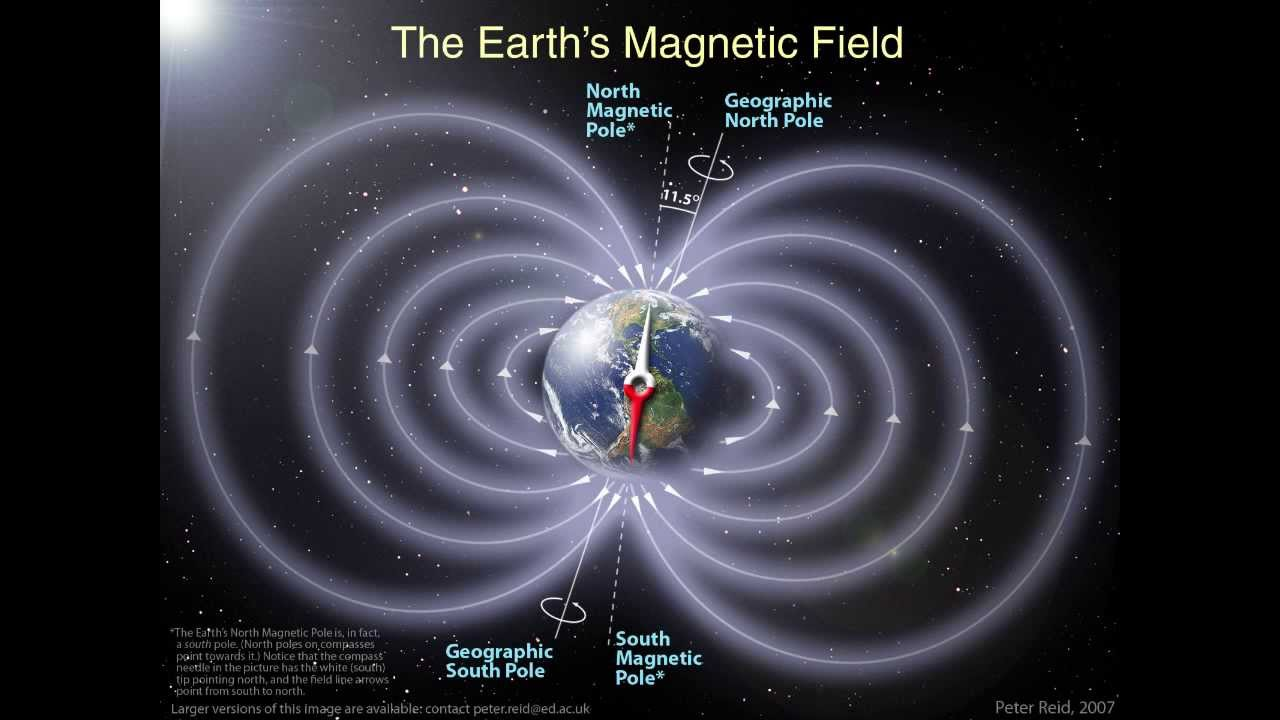
\includegraphics[width=\linewidth]{maxresdefault.jpg}
  \caption{The Earth's Magnetic Field.}
  \label{fig:magField}
   \cite{magEarth}
\end{figure}

\section*{Japanese scientific activities in space research}
Japan launched several satellites in the past and will continue to launch in future. In 1989 and 1992, the satellites, Akebono and Geotail, to the space. Akebono's mission finished in 2015. In 2016, ERG(Arase) was launched and it is operating in the space. In 1998, Japan launched Nozomi to the Mars, but the mission failed. In 2007, Japan successfully launched Kaguya to the Moon. In this year, BepiColombo/MMO will be launched to the Mercury by the project which is operated by the collaboration by Japan and EU\cite{lecture}.\\
After several years of service, Akebono provided a large numbers of space data. It contained several instrunments such as, DC Magnetic Field, DC Electric Field, Ion \& Electron Detector, High Frequency Wave Receiver (20kHz - 5MHz), Low Frequency Wave Receiver (0 - 20kHz) and Visible and UV Auroal Image. By using Low Frequency Wave Receiver, approximately 1.5 TBytes of digital data was received and stored in 28,000 tapes of Analog Waveform data (approximately 20TBytes)\cite{lecture}.\\

\section*{Intellgent Signal Processing Onboard Spacecraft System}
\paragraph*{How to send the data to the ground:} There are magnetic sensors that are installed on the instrument. This sensors measure the space magnetic environment and send the information to the receiver which is also located in the instrunment. Then the reciever processes on the raw data to send back to the earth. Before sending, the raw data was processed by onboard CPU such operation as compressing the data and so on and then send the data back to the earth. The tracking sataion then recieves the data send to the databse. The ground data process is done at the final step\cite{lecture}.\\
For Bepi Colombo Mission, there are some interesting things. The distance is so far from the earth and the ground crews must make sure that the satellite can operate properly. More importantly, the data from the satellite should be successfully sent to the earth. There are three modes: LOW-mode, Medium-mode, and High-mode which have 0.5kbps/ave, 1.0kbps/ave, and 1.0kbps/ave. So we can see that it will be very difficult to obtain many data with this kind of data transfer rate\cite{lecture}.\\
That is the reason that Mission Data Processing (MDP) software is very important. The data storage in the MDP will be divided into many ring-buffers. One long buffer and one short buffer will be allocated to each sensor. In nominal, mission data will be stored in the long buffers and "L/M mode" data will be produced. In "H-mode" operation, data in the long buffers will be preserved for data production of "H mode" data and short buffers ($\sim$12s) will be used for the continuous "L/M mode" data production\cite{lecture}.\\
\section*{SCOPE Mission}
This mission is formation flying satellites that contains one mother satellite, one daughter satellite (near distance of 10 $\sim$ 100km), and three daughter satellites (far distance of 100 $\sim$ 5000km). This is the Co-operational observating using Inter-satellite commuication system. So network configuration of the simulator is used to test various environments. There will be three satellite PCs which are one mother satellite and two daughter satellites. Another PC is to simulate the space.\\
\section*{How to make spacecraft}
It is very important that the electronic equipments survive in the space environment. The rate of changes of temperature in the space is very high in the space. So it is very important that the heat which is produced from the electronic equipment must be as low as possible. To make sure that the equipments are resistant to the high temperatue, the equipments must pass several tests on the ground. Another problem is the vibration at launching and operation. The equipments must be tested for the vibrations test. After several tests, the equipments are moved to the launch site and tested again. After final function test at launch site, the satellite is put in the spacecraft and fairing assembly. Finally, the satellite is launched to the space by using rocket\cite{lecture}.



